\documentclass[]{beamer}
\usepackage{tikz}
\usepackage{pgfplots}
\usepackage[dutch]{babel}
\usepackage[T1]{fontenc}
\usepackage{graphicx}
\usepackage{braket}
\usepackage{color}
\usepackage{xcolor}
\usepackage{wrapfig}
\usepackage{amsmath}
\usepackage{listings}
\usepackage{wasysym}
\usepackage{tikz}

\usepackage[active,tightpage,pdftex]{preview}

\renewcommand{\thefootnote}{}
\addtolength{\jot}{1em}
\renewcommand{\familydefault}{\sfdefault}
\renewcommand*\sfdefault{lmss}

\definecolor{green}{rgb}{0.24,0.60,0.34}
\definecolor{purple}{rgb}{0.60,0.24,0.44}

\newsavebox\MBox
\newcommand\Cline[2][red]{{\sbox\MBox{$#2$}%
  \rlap{\usebox\MBox}\color{#1}\rule[-1.2\dp\MBox]{\wd\MBox}{0.5pt}}}

\makeatletter
\def\beamer@origitem{%
  \@inmatherr\item\@ifnextchar[\@item{\@noitemargtrue\@item[\@itemlabel]%
  \csname beamer@thcfg@\beameritemnestingprefix item\endcsname% Insert colour in \beamer@thc@fg
  \ifx\beamer@thc@fg\@empty\relax\else\color{\beamer@thc@fg}\fi% Execute colour
 }}
\makeatother


% TITLE PAGE
\title[]{
Light-weight tools for clustering and classification by file compression} % The short title appears at the bottom of every slide, the full title is only on the title page

\author{Geert Kapteijns} % Your name
\institute[CWI] % Your institution as it will appear on the bottom of every slide, may be shorthand to save space
{
Universiteit van Amsterdam \\ % Your institution for the title page
\medskip
}
\date{\today} % Date, can be changed to a custom date



\begin{document}
\setbeamercolor{frametitle}{fg=white,bg=black}

\setbeamercolor{background canvas}{bg=black}
\setbeamercolor{frametitle}{fg=black,bg=white}
\setbeamercolor{footnote}{fg=white}
\setbeamercolor{footnote mark}{fg=white}
\setbeamertemplate{navigation symbols}{}%remove navigation symbols
\color{white}
\setbeamercolor{itemize item}{fg=white}
\setbeamercolor{item}{fg=white}

\setbeamercolor{normal text}{fg=white,bg=white}
\setbeamercolor{alerted text}{fg=white}
\setbeamercolor{example text}{fg=white}
\setbeamercolor{structure}{fg=white}

\setbeamercolor{palette primary}{fg=white}
\setbeamercolor{palette secondary}{fg=white}
\setbeamercolor{palette tertiary}{fg=white}
\setbeamercolor{palette quaternary}{fg=white}

\setbeamercolor{author}{fg=white}
\setbeamercolor{date}{fg=white}
\setbeamercolor{institute}{fg=white}

\usetikzlibrary{arrows}



\begin{frame}
  \titlepage
\end{frame}

\begin{frame}
  % \colorbox{white}{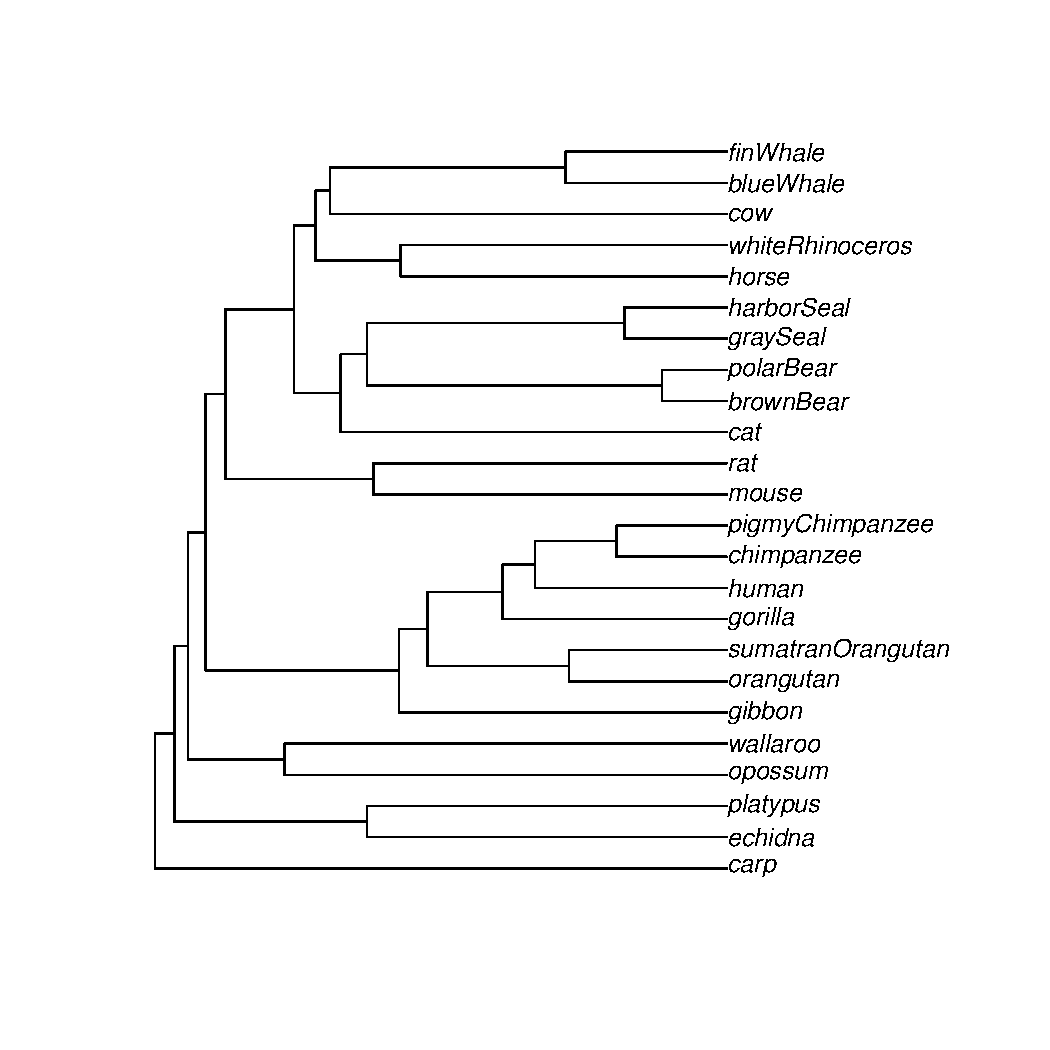
\includegraphics[width=\textwidth]{thesis/Pictures/24-mammals-average.pdf}}
  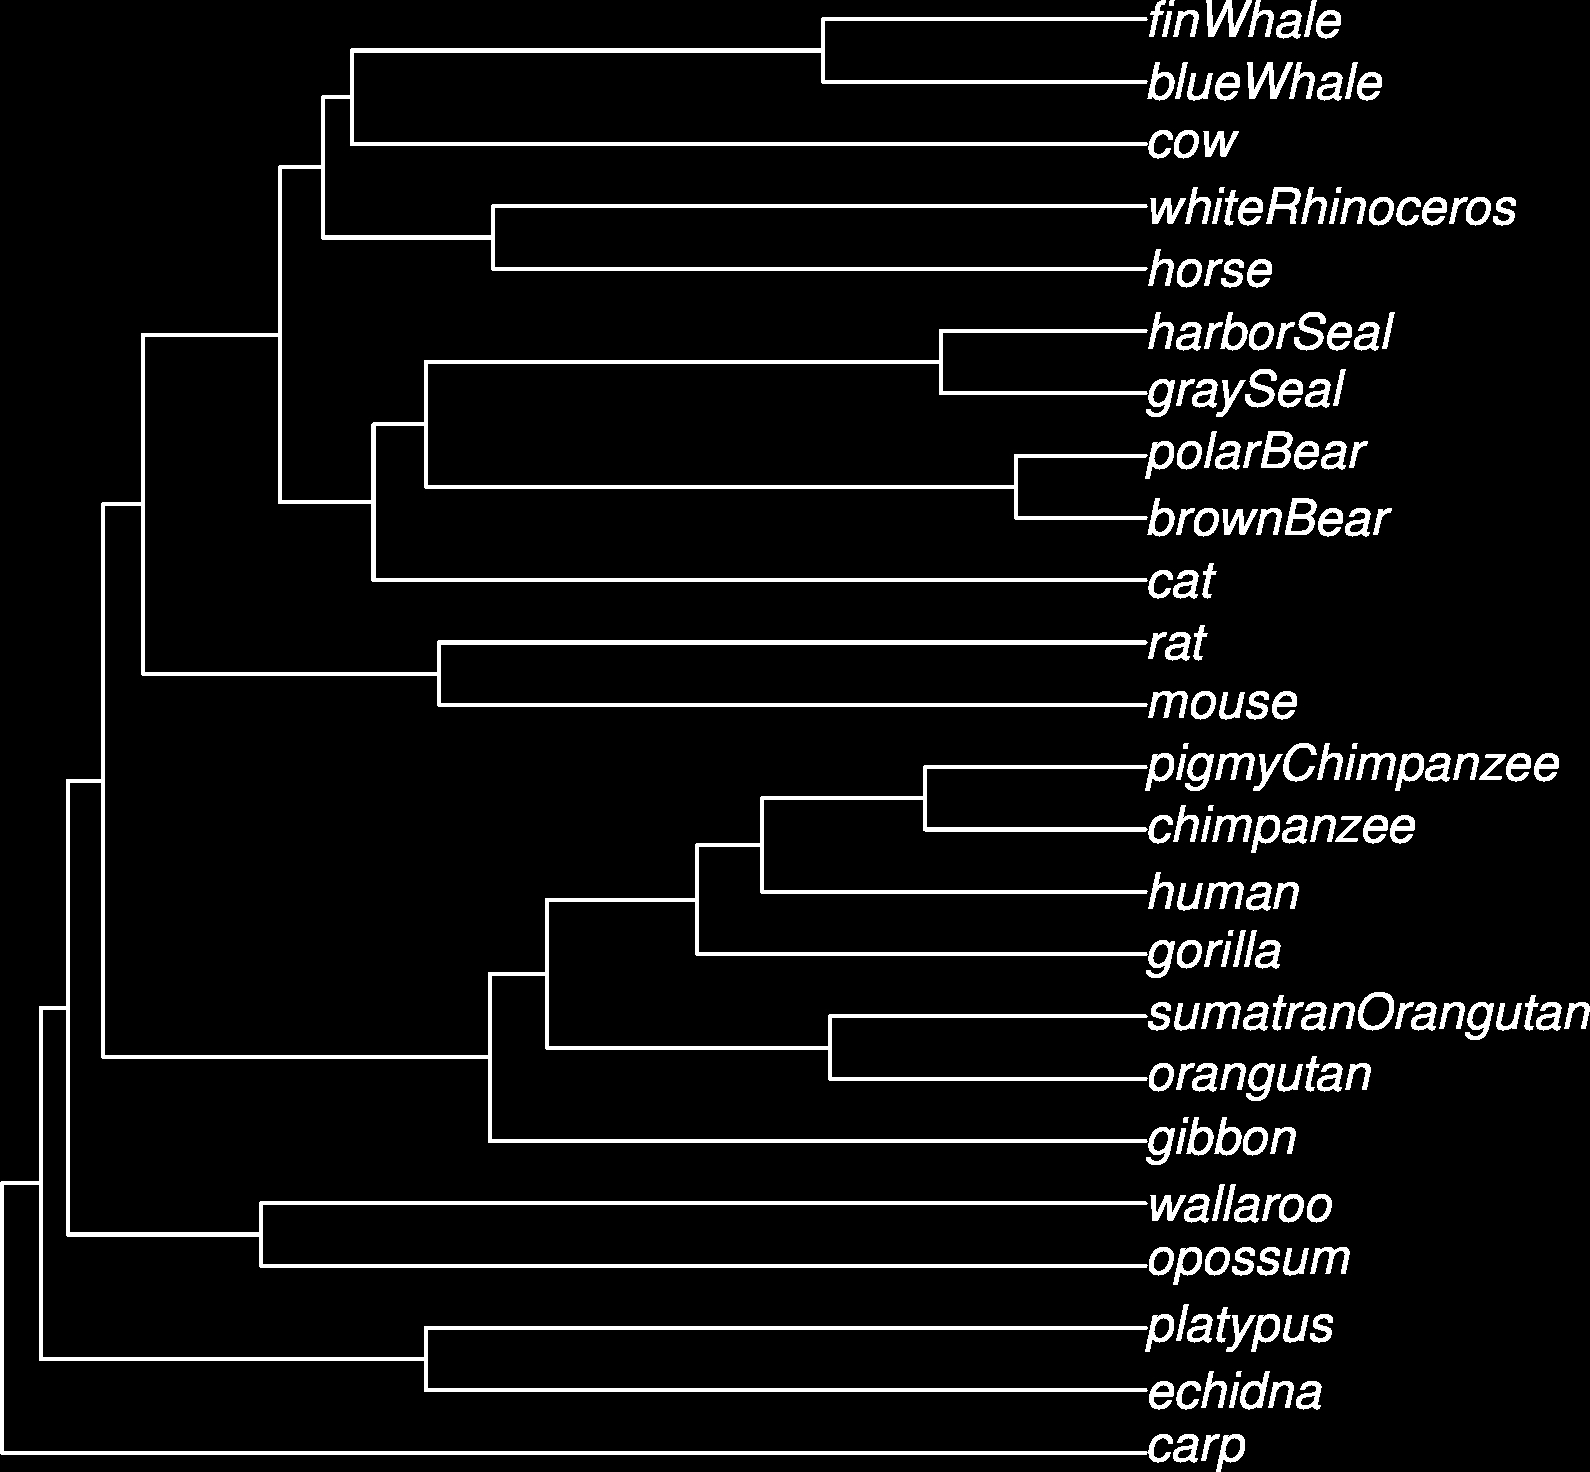
\includegraphics[scale=0.16]{thesis/Pictures/24-mammals-average-negated.jpg}
\end{frame}

\begin{frame}
  \texttt{A	T	G	C	C	G	T	T	A	G	A	C	C	G	T	T	A	G	C	G	G	A	C	C	T	G	A}\\
  \texttt{C C C G A G C G G C G C A A C C G A T T A G T C T T C}
\end{frame}

\begin{frame}
  \texttt{0000000000000000000000000000000000000000\\
          0000000000000000000000000000000000000000\\
          0000000000000000000000000000000000000000\\
          0000000000000000000000000000000000000000}
\end{frame}

\begin{frame}[fragile]
    \begin{lstlisting}[language=Ruby]
      160.times { puts "0" }
    \end{lstlisting}
\end{frame}

\begin{frame}
  \texttt{0010110110000011010110001000101010100111\\
          1010101001100001111010000010011111010010\\
          0100100000000110001101101111001111001101\\
          1011100110101111010111110001110111000101}
\end{frame}

\begin{frame}
  $2^n$ strings van lengte $n$.

  $$1 + 2 + 4 + \dots + 2^{n-1} = 2^n - 1$$

  $2^n - 1$ kortere beschrijvingen.
\end{frame}

\begin{frame}
  \texttt{0010010000111111011010101000100010000101\\
          1010001100001000110100110001001100011001\\
          1000101000101110000000110111000001110011\\
          0100010010100100000010010011100000100010}\\~\\

  \pause
  $\pi$ in binary!
\end{frame}

\begin{frame}
  $$\frac1{\pi} = \frac{2\sqrt{2}}{9801} \sum_{k=0}^\infty \frac{(4k)!(1103+26390k)}{(k!)^4 396^{4k}}\!$$
  (Ramanujan)
\end{frame}

\begin{frame}[fragile]
  \begin{lstlisting}[language=Ruby]
    # N bits.
    def kolmogorov_complexity(string)
      # ...
    end
  \end{lstlisting}

  \pause

  \begin{lstlisting}[language=Ruby]
    # lexographical ordering
    all_strings.each do |string|
      if kolmogorov_complexity(string) > M
        puts string
      end
    end
  \end{lstlisting}

  \pause

  $$ M > N + \epsilon $$
\end{frame}

\begin{frame}
   $$K(x|y)$$
\end{frame}

\begin{frame}
  $$\text{NID}(x, y) = \frac{\max \{ K(x|y), K(y|x) \}}{\max \{ K(x), K(y)\}}$$
\end{frame}

\begin{frame}
  $$\text{NID}(x,y) \leq d(x,y) + \mathcal{O}(\frac{1}{K})$$
\end{frame}

\begin{frame}
  $$\text{NCD} = \frac{C(xy) - \min \{ C(x), C(y) \}}{\max \{ C(x), C(y) \}}$$
\end{frame}

\begin{frame}
  % \colorbox{white}{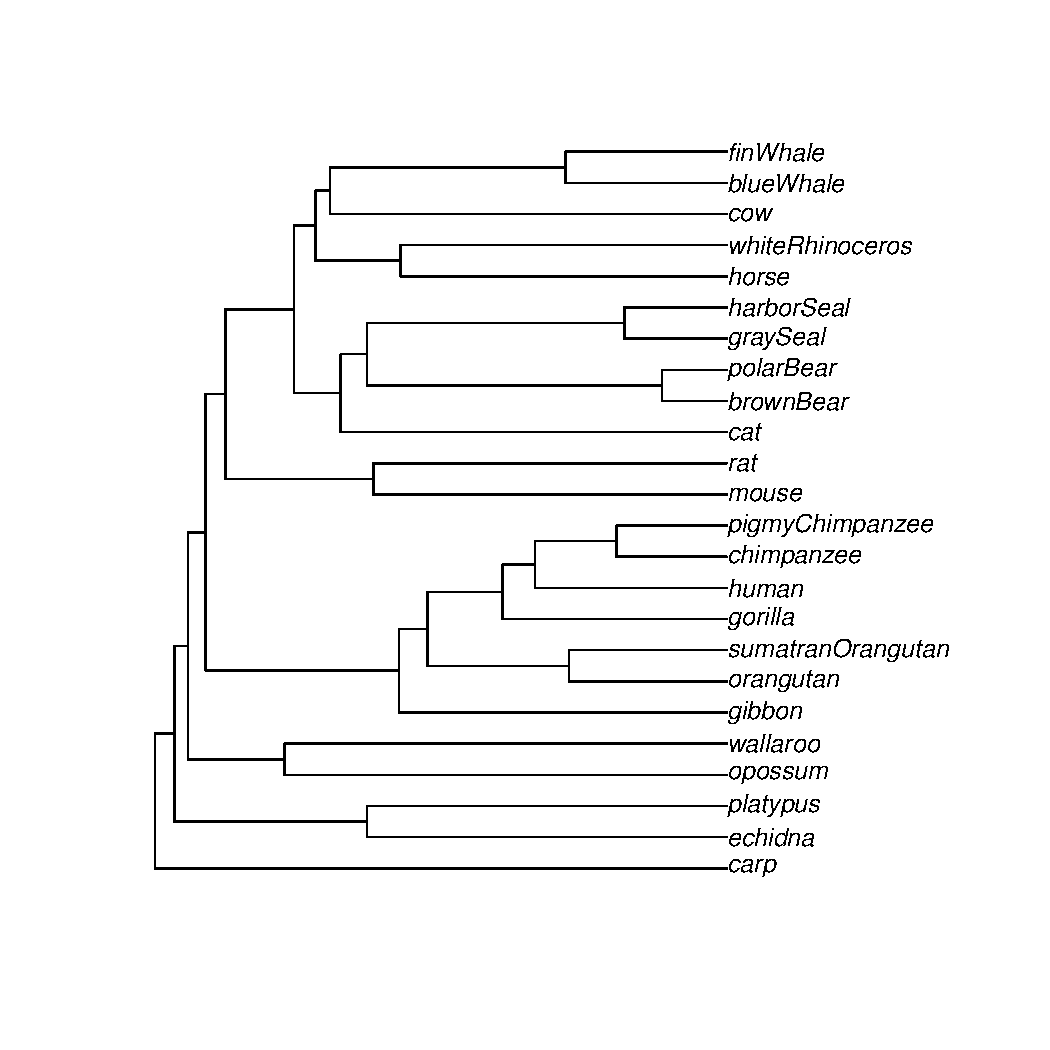
\includegraphics[width=\textwidth]{thesis/Pictures/24-mammals-average.pdf}}
  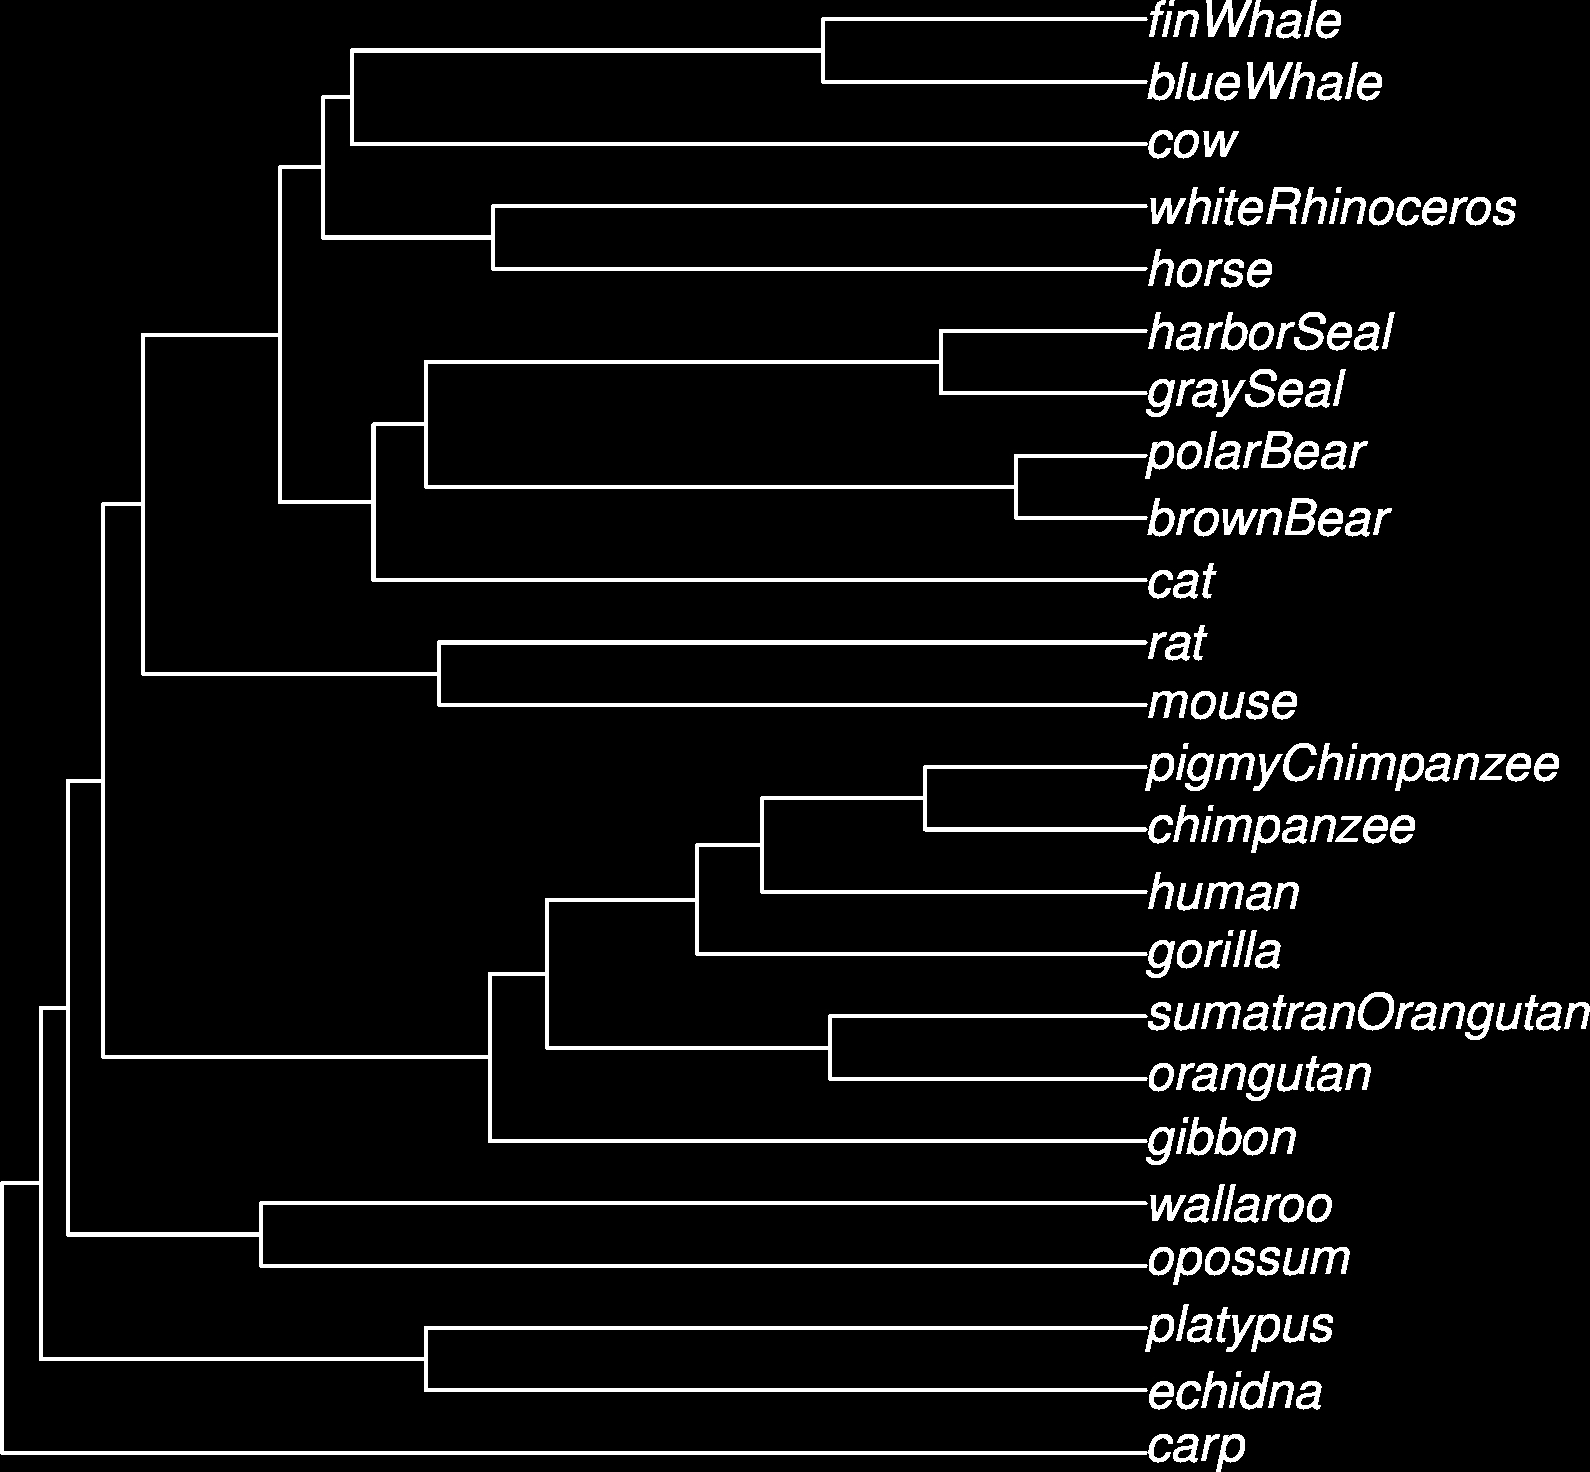
\includegraphics[scale=0.16]{thesis/Pictures/24-mammals-average-negated.jpg}
\end{frame}

\begin{frame}

  \begin{displaymath}
    \begin{bmatrix}
      \text{gemiddeld aantal woorden per zin} \\
      \text{aantal leestekens} \\
      \text{aantal keer dat \textit{linux} voorkomt}

    \end{bmatrix}
    \pause
    =
    \begin{bmatrix}
      \text{8.3} \\
      \text{1.8} \\
      \text{3}

    \end{bmatrix}
  \end{displaymath}

\end{frame}

\begin{frame}

  \begin{tikzpicture}[>=stealth']
    % Draw axes
    \draw [<->,thick] (0,5) node (yaxis) [above] {feature 2}
          |- (5,0) node (xaxis) [right] {feature 1};
    % draw line
    \draw (0,-1) -- (5,4); % y=x-1
    \draw[dashed] (-1,0) -- (4,5); % y=x+1
    \draw[dashed] (2,-1) -- (6,3); % y=x-3
    % \draw labels
    % \draw (3.5,3) node[rotate=45,font=\small]
    %       {$\mathbf{w}\cdot \mathbf{x} + b = 0$};
    % \draw (2.5,4) node[rotate=45,font=\small]
    %       {$\mathbf{w}\cdot \mathbf{x} + b = 1$};
    % \draw (4.5,2) node[rotate=45,font=\small]
    %       {$\mathbf{w}\cdot \mathbf{x} + b = -1$};
    % draw distance
    % \draw[dotted] (4,5) -- (6,3);
    % \draw (5.25,4.25) node[rotate=-45] {$\frac{2}{\Vert \mathbf{w} \Vert}$};
    % \draw[dotted] (0,0) -- (0.5,-0.5);
    % \draw (0,-0.5) node[rotate=-45] {$\frac{b}{\Vert \mathbf{w} \Vert}$};
    \draw[->] (2,1) -- (1, 2);
    % \draw (1.85,1.35) node[rotate=-45] {$\mathbf{w}$};
    % draw negative dots
    % \fill[red] (0.5,1.5) circle (3pt);
    \fill[red]   (1.5,2.5)   circle (3pt);
    \fill[white] (1,2.5)     circle (3pt);
    \fill[white] (0.75,2)    circle (3pt);
    \fill[white] (0.6,1.9)   circle (3pt);
    \fill[white] (0.77, 2.5) circle (3pt);
    \fill[white] (1.5,3)     circle (3pt);
    \fill[white] (1.3,3.3)   circle (3pt);
    \fill[white] (0.6,3.2)   circle (3pt);
    % draw positive dots
    % \draw[red,thick] (4,1)     circle (3pt);
    \draw[red,thick] (3.3,.3)  circle (3pt);
    \draw[white]     (4.5,1.2) circle (3pt);
    \draw[white]     (4.5,.5)  circle (3pt);
    \draw[white]     (3.9,.7)  circle (3pt);
    \draw[white]     (5,1)     circle (3pt);
    \draw[white]     (3.5,.2)  circle (3pt);
    \draw[white]     (4,.3)    circle (3pt);

    \pause

    \fill[green]     (1.1, 1.2)    circle(3pt);
  \end{tikzpicture}

\end{frame}




\end{document}
